% Practice Test 05 — Virginia Edition
% Questions: 30 (25 MC + 5 SA)
% Generated by scripts/generate_practice_tests.py

\begin{practiceQuestion}{1-4-q04}{mc}
\begin{questionText}
A recipe uses $\frac{3}{4}$ cup of flour per serving. How much flour $f$ is needed for $s$ servings?
\end{questionText}
\choiceA{$f = \frac{3}{4}s$}
\choiceB{$f = \frac{4}{3}s$}
\choiceC{$f = s - \frac{3}{4}$}
\choiceD{$f = \frac{s}{3}$}
\correctAnswer{A}
\explanation{Each serving uses $\frac{3}{4}$ cup, so total flour $= \frac{3}{4} \times$ servings, giving $f = \frac{3}{4}s$.}
\end{practiceQuestion}

\begin{practiceQuestion}{2-1-q15}{mc}
\begin{questionText}
A library has $480$ books. If $35\%$ are fiction, how many fiction books does the library have?
\end{questionText}
\choiceA{$148$}
\choiceB{$160$}
\choiceC{$168$}
\choiceD{$172$}
\correctAnswer{C}
\explanation{$35\% = 0.35$. Multiply: $0.35 \times 480 = 168$ fiction books.}
\end{practiceQuestion}

\begin{practiceQuestion}{2-2-q06}{mc}
\begin{questionText}
In a bag of $150$ marbles, $60$ are blue. What percent of the marbles are blue?
\end{questionText}
\choiceA{$25\%$}
\choiceB{$30\%$}
\choiceC{$35\%$}
\choiceD{$40\%$}
\correctAnswer{D}
\explanation{$\frac{60}{150} = \frac{p}{100}$. Cross-multiply: $150p = 6000$. Divide: $p = 40\%$.}
\end{practiceQuestion}

\begin{practiceQuestion}{2-3-q24}{sa}
\begin{questionText}
A town's population increased by $8\%$ from $25{,}000$. What is the new population?
\end{questionText}
\correctAnswer{$27{,}000$}
\explanation{$25{,}000 \times 1.08 = 27{,}000$.}
\end{practiceQuestion}

\begin{practiceQuestion}{2-7-q27}{gmc}
\begin{questionText}
The bar graph shows the estimated and actual heights of three trees. Which tree has the greatest percent error?

\begin{center}
\begin{tikzpicture}[scale=0.5]
  \draw[thick,->] (0,0) -- (0,7) node[above]{\small Height (ft)};
  \draw[thick,->] (0,0) -- (10.5,0);
  % Tree A: est 20, actual 25
  \fill[funBlue!60] (0.5,0) rectangle (1.5,4);
  \fill[funGreen!60] (1.5,0) rectangle (2.5,5);
  % Tree B: est 15, actual 12
  \fill[funBlue!60] (3.5,0) rectangle (4.5,3);
  \fill[funGreen!60] (4.5,0) rectangle (5.5,2.4);
  % Tree C: est 30, actual 28
  \fill[funBlue!60] (6.5,0) rectangle (7.5,6);
  \fill[funGreen!60] (7.5,0) rectangle (8.5,5.6);
  % Labels
  \node[below,font=\small] at (1.5,0) {Tree A};
  \node[below,font=\small] at (4.5,0) {Tree B};
  \node[below,font=\small] at (7.5,0) {Tree C};
  \foreach \y/\lab in {1/5,2/10,3/15,4/20,5/25,6/30} {
    \draw (-0.1,\y) -- (0.1,\y) node[left,font=\small,xshift=-2pt] {\lab};
  }
  % Values
  \node[above,font=\scriptsize,funBlue] at (1,4) {$20$};
  \node[above,font=\scriptsize,funGreen!80!black] at (2,5) {$25$};
  \node[above,font=\scriptsize,funBlue] at (4,3) {$15$};
  \node[above,font=\scriptsize,funGreen!80!black] at (5,2.4) {$12$};
  \node[above,font=\scriptsize,funBlue] at (7,6) {$30$};
  \node[above,font=\scriptsize,funGreen!80!black] at (8,5.6) {$28$};
  % Legend
  \fill[funBlue!60] (0.5,6.8) rectangle (1,7.2);
  \node[right,font=\scriptsize] at (1.1,7) {Estimated};
  \fill[funGreen!60] (3.5,6.8) rectangle (4,7.2);
  \node[right,font=\scriptsize] at (4.1,7) {Actual};
\end{tikzpicture}
\end{center}
\end{questionText}
\choiceA{Tree A ($20\%$)}
\choiceB{Tree B ($25\%$)}
\choiceC{Tree C ($7.1\%$)}
\choiceD{Trees A and B are tied}
\correctAnswer{B}
\explanation{A: $|20-25|/25 = 20\%$. B: $|15-12|/12 = 25\%$. C: $|30-28|/28 \approx 7.1\%$. Tree B has the greatest error.}
\end{practiceQuestion}

\begin{practiceQuestion}{3-2-q16}{mc}
\begin{questionText}
When you add two negative integers, the result is always:
\end{questionText}
\choiceA{Positive}
\choiceB{Zero}
\choiceC{Negative}
\choiceD{It depends on the numbers}
\correctAnswer{C}
\explanation{Adding two negative integers gives a negative sum. Same signs: add absolute values and keep the negative sign.}
\end{practiceQuestion}

\begin{practiceQuestion}{3-3-q10}{mc}
\begin{questionText}
What is $0 - (-6)$?
\end{questionText}
\choiceA{$-6$}
\choiceB{$6$}
\choiceC{$0$}
\choiceD{$-12$}
\correctAnswer{B}
\explanation{$0 - (-6) = 0 + 6 = 6$. Subtracting a negative is the same as adding.}
\end{practiceQuestion}

\begin{practiceQuestion}{3-4-q28}{gmc}
\begin{questionText}
Look at the table of a scuba diver's depth changes.

\begin{center}
\begin{tabular}{|c|c|}
\hline
\textbf{Action} & \textbf{Change (meters)} \\
\hline
Start & $-8.5$ \\
\hline
Dive deeper & $-3.2$ \\
\hline
Rise up & $+6.4$ \\
\hline
\end{tabular}
\end{center}

What is the diver's final depth?
\end{questionText}
\choiceA{$-18.1$ m}
\choiceB{$-5.3$ m}
\choiceC{$-11.7$ m}
\choiceD{$1.3$ m}
\correctAnswer{B}
\explanation{$-8.5 + (-3.2) + 6.4 = -11.7 + 6.4 = -5.3$ m.}
\end{practiceQuestion}

\begin{practiceQuestion}{4-3-q13}{mc}
\begin{questionText}
Expand and simplify $-2(3x + 1) + 4(x - 3)$.
\end{questionText}
\choiceA{$-2x - 14$}
\choiceB{$-2x + 14$}
\choiceC{$2x - 14$}
\choiceD{$-2x - 10$}
\correctAnswer{A}
\explanation{Expand: $-6x - 2 + 4x - 12$. Combine: $(-6x + 4x) + (-2 - 12) = -2x - 14$.}
\end{practiceQuestion}

\begin{practiceQuestion}{4-4-q01}{mc}
\begin{questionText}
What is the greatest common factor (GCF) of $12$ and $18$?
\end{questionText}
\choiceA{$2$}
\choiceB{$3$}
\choiceC{$6$}
\choiceD{$9$}
\correctAnswer{C}
\explanation{Factors of $12$: $1, 2, 3, 4, 6, 12$. Factors of $18$: $1, 2, 3, 6, 9, 18$. The greatest common factor is $6$.}
\end{practiceQuestion}

\begin{practiceQuestion}{5-4-q03}{mc}
\begin{questionText}
Solve $0.25n - 1.5 = 3.5$.
\end{questionText}
\choiceA{$n = 8$}
\choiceB{$n = 20$}
\choiceC{$n = 14$}
\choiceD{$n = 2$}
\correctAnswer{B}
\explanation{Add $1.5$: $0.25n = 5$. Divide by $0.25$: $n = 20$. Check: $0.25(20) - 1.5 = 5 - 1.5 = 3.5$ \checkmark.}
\end{practiceQuestion}

\begin{practiceQuestion}{5-5-q08}{mc}
\begin{questionText}
Solve $\dfrac{x}{3} + 4 < 10$.
\end{questionText}
\choiceA{$x < 18$}
\choiceB{$x < 42$}
\choiceC{$x < 2$}
\choiceD{$x < 6$}
\correctAnswer{A}
\explanation{Subtract $4$: $\frac{x}{3} < 6$. Multiply by $3$: $x < 18$.}
\end{practiceQuestion}

\begin{practiceQuestion}{5-6-q18}{mc}
\begin{questionText}
Solve $6 - 2x \leq -4$ and describe the graph.
\end{questionText}
\choiceA{Closed circle at $5$, shade right}
\choiceB{Open circle at $5$, shade right}
\choiceC{Closed circle at $5$, shade left}
\choiceD{Closed circle at $-5$, shade right}
\correctAnswer{A}
\explanation{Subtract $6$: $-2x \leq -10$. Divide by $-2$ and flip: $x \geq 5$. Closed circle at $5$, shade right.}
\end{practiceQuestion}

\begin{practiceQuestion}{6-1-q29}{gsa}
\begin{questionText}
The scale drawing below shows an L-shaped room. The scale is $1$ cm $= 2$ m. What is the actual area of the room?

\begin{center}
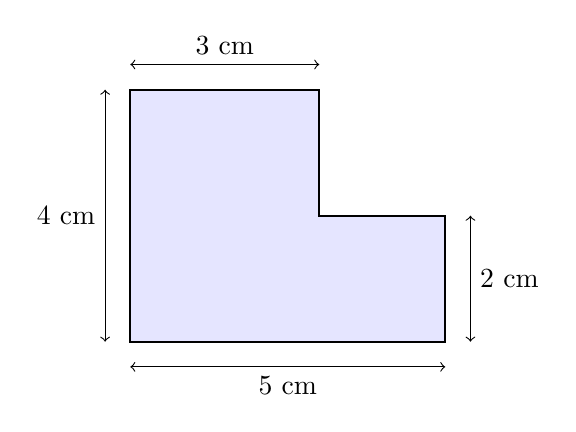
\begin{tikzpicture}[scale=0.8]
  \draw[thick,fill=blue!10] (0,0) -- (5,0) -- (5,2) -- (3,2) -- (3,4) -- (0,4) -- cycle;
  \draw[<->] (0,-0.4) -- (5,-0.4);
  \node[below] at (2.5,-0.4) {$5$ cm};
  \draw[<->] (5.4,0) -- (5.4,2);
  \node[right] at (5.4,1) {$2$ cm};
  \draw[<->] (-0.4,0) -- (-0.4,4);
  \node[left] at (-0.4,2) {$4$ cm};
  \draw[<->] (0,4.4) -- (3,4.4);
  \node[above] at (1.5,4.4) {$3$ cm};
\end{tikzpicture}
\end{center}
\end{questionText}
\correctAnswer{$64$ m$^2$}
\explanation{Split into two rectangles. Left: $3$ cm $\times$ $4$ cm $= 12$ cm$^2$. Bottom-right: $(5-3)$ cm $\times$ $2$ cm $= 4$ cm$^2$. Total drawing area: $16$ cm$^2$. Scale: $1$ cm $= 2$ m, so areas scale by $2^2 = 4$. Actual area: $16 \times 4 = 64$ m$^2$.}
\end{practiceQuestion}

\begin{practiceQuestion}{6-2-q17}{mc}
\begin{questionText}
A map uses $1$ cm $= 60$ km. You redraw it at $1$ cm $= 20$ km. A triangle on the original has an area of $4$ cm$^2$. What is its area on the new map?
\end{questionText}
\choiceA{$12$ cm$^2$}
\choiceB{$16$ cm$^2$}
\choiceC{$36$ cm$^2$}
\choiceD{$48$ cm$^2$}
\correctAnswer{C}
\explanation{Scale ratio: $\frac{60}{20} = 3$. Area scales by $3^2 = 9$. New area: $4 \times 9 = 36$ cm$^2$.}
\end{practiceQuestion}

\begin{practiceQuestion}{6-5-q08}{mc}
\begin{questionText}
A cylinder is sliced with a vertical cut through its center, perpendicular to the base. What shape is the cross-section?
\end{questionText}
\choiceA{Circle}
\choiceB{Rectangle}
\choiceC{Oval}
\choiceD{Triangle}
\correctAnswer{B}
\explanation{A vertical cut through the center of a cylinder produces a rectangle. The width equals the diameter and the height equals the cylinder's height.}
\end{practiceQuestion}

\begin{practiceQuestion}{6-6-q08}{mc}
\begin{questionText}
An angle measures $38°$. Its complement measures:
\end{questionText}
\choiceA{$38°$}
\choiceB{$52°$}
\choiceC{$142°$}
\choiceD{$322°$}
\correctAnswer{B}
\explanation{Complementary angles sum to $90°$. $90° - 38° = 52°$.}
\end{practiceQuestion}

\begin{practiceQuestion}{6-7-q25}{sa}
\begin{questionText}
What single transformation maps $(x, y)$ to $(-x, -y)$?
\end{questionText}
\correctAnswer{A $180°$ rotation about the origin}
\explanation{Negating both coordinates is equivalent to rotating $180°$ about the origin. It is also equivalent to reflecting over both axes.}
\end{practiceQuestion}

\begin{practiceQuestion}{6-8-q02}{mc}
\begin{questionText}
Two similar rectangles have corresponding sides $5$ cm and $15$ cm. If the shorter rectangle has a width of $3$ cm, what is the width of the larger rectangle?
\end{questionText}
\choiceA{$6$ cm}
\choiceB{$9$ cm}
\choiceC{$13$ cm}
\choiceD{$45$ cm}
\correctAnswer{B}
\explanation{Scale factor: $\frac{15}{5} = 3$. Width of larger: $3 \times 3 = 9$ cm.}
\end{practiceQuestion}

\begin{practiceQuestion}{7-4-q10}{mc}
\begin{questionText}
A figure is made of a trapezoid with parallel sides $6$ cm and $10$ cm, and height $4$ cm. Which expression gives its area?
\end{questionText}
\choiceA{$6 \times 10 \times 4$}
\choiceB{$\frac{1}{2} \times 6 \times 10$}
\choiceC{$\frac{1}{2} \times (6 + 10) \times 4$}
\choiceD{$(6 + 10) \times 4$}
\correctAnswer{C}
\explanation{Area of a trapezoid $= \frac{1}{2}(b_1 + b_2) \times h = \frac{1}{2}(6 + 10) \times 4 = 32$ cm$^2$.}
\end{practiceQuestion}

\begin{practiceQuestion}{7-5-q10}{mc}
\begin{questionText}
A cube has a surface area of $54$ cm$^2$. What is the area of one face?
\end{questionText}
\choiceA{$6$ cm$^2$}
\choiceB{$9$ cm$^2$}
\choiceC{$18$ cm$^2$}
\choiceD{$27$ cm$^2$}
\correctAnswer{B}
\explanation{A cube has $6$ identical faces. Area of one face $= 54 \div 6 = 9$ cm$^2$.}
\end{practiceQuestion}

\begin{practiceQuestion}{7-6-q18}{mc}
\begin{questionText}
A trapezoidal prism has a trapezoidal base with parallel sides $4$ cm and $6$ cm, height $3$ cm, and the prism length is $10$ cm. What is its volume?
\end{questionText}
\choiceA{$60$ cm$^3$}
\choiceB{$120$ cm$^3$}
\choiceC{$150$ cm$^3$}
\choiceD{$180$ cm$^3$}
\correctAnswer{C}
\explanation{$B = \frac{1}{2}(4 + 6) \times 3 = 15$ cm$^2$. $V = 15 \times 10 = 150$ cm$^3$.}
\end{practiceQuestion}

\begin{practiceQuestion}{7-7-q11}{mc}
\begin{questionText}
If you double the radius of a cylinder but keep the height the same, what happens to the volume?
\end{questionText}
\choiceA{It doubles}
\choiceB{It triples}
\choiceC{It quadruples}
\choiceD{It increases by a factor of $8$}
\correctAnswer{C}
\explanation{$V = \pi r^2 h$. If $r$ becomes $2r$, then $V = \pi(2r)^2 h = 4\pi r^2 h$. The volume quadruples.}
\end{practiceQuestion}

\begin{practiceQuestion}{8-1-q08}{mc}
\begin{questionText}
A sample of $40$ out of $2{,}000$ voters is surveyed. What fraction of the population is in the sample?
\end{questionText}
\choiceA{$\frac{1}{50}$}
\choiceB{$\frac{1}{40}$}
\choiceC{$\frac{1}{20}$}
\choiceD{$\frac{1}{500}$}
\correctAnswer{A}
\explanation{$\frac{40}{2{,}000} = \frac{1}{50}$.}
\end{practiceQuestion}

\begin{practiceQuestion}{8-3-q30}{gsa}
\begin{questionText}
The dot plots show quiz scores for two classes (out of $10$).

\begin{center}
\begin{tikzpicture}[scale=0.6]
  % Class X
  \node[left,font=\small\bfseries] at (3.5,2) {Class X};
  \draw[thick,->] (3.5,0) -- (11.5,0);
  \foreach \x in {4,5,...,10} {
    \draw (\x,0.1) -- (\x,-0.1);
    \node[below,font=\small] at (\x,0) {$\x$};
  }
  % Class X data: 5(1),6(2),7(4),8(5),9(3),10(1) = 16 students
  \fill[funBlue] (5,0.35) circle (0.13);
  \fill[funBlue] (6,0.35) circle (0.13); \fill[funBlue] (6,0.65) circle (0.13);
  \fill[funBlue] (7,0.35) circle (0.13); \fill[funBlue] (7,0.65) circle (0.13); \fill[funBlue] (7,0.95) circle (0.13); \fill[funBlue] (7,1.25) circle (0.13);
  \fill[funBlue] (8,0.35) circle (0.13); \fill[funBlue] (8,0.65) circle (0.13); \fill[funBlue] (8,0.95) circle (0.13); \fill[funBlue] (8,1.25) circle (0.13); \fill[funBlue] (8,1.55) circle (0.13);
  \fill[funBlue] (9,0.35) circle (0.13); \fill[funBlue] (9,0.65) circle (0.13); \fill[funBlue] (9,0.95) circle (0.13);
  \fill[funBlue] (10,0.35) circle (0.13);

  % Class Y
  \node[left,font=\small\bfseries] at (3.5,5.5) {Class Y};
  \draw[thick,->] (3.5,3.5) -- (11.5,3.5);
  \foreach \x in {4,5,...,10} {
    \draw (\x,3.6) -- (\x,3.4);
  }
  % Class Y data: 4(2),5(3),6(4),7(3),8(2),9(1),10(1) = 16 students
  \fill[funGreen] (4,3.85) circle (0.13); \fill[funGreen] (4,4.15) circle (0.13);
  \fill[funGreen] (5,3.85) circle (0.13); \fill[funGreen] (5,4.15) circle (0.13); \fill[funGreen] (5,4.45) circle (0.13);
  \fill[funGreen] (6,3.85) circle (0.13); \fill[funGreen] (6,4.15) circle (0.13); \fill[funGreen] (6,4.45) circle (0.13); \fill[funGreen] (6,4.75) circle (0.13);
  \fill[funGreen] (7,3.85) circle (0.13); \fill[funGreen] (7,4.15) circle (0.13); \fill[funGreen] (7,4.45) circle (0.13);
  \fill[funGreen] (8,3.85) circle (0.13); \fill[funGreen] (8,4.15) circle (0.13);
  \fill[funGreen] (9,3.85) circle (0.13);
  \fill[funGreen] (10,3.85) circle (0.13);
\end{tikzpicture}
\end{center}

Find the mean score for each class and determine which class performed better on the quiz.
\end{questionText}
\correctAnswer{Class X mean $\approx 7.75$; Class Y mean $\approx 6.25$. Class X performed better.}
\explanation{Class X: $(5+12+28+40+27+10) \div 16 = 122 \div 16 \approx 7.63$. Class Y: $(8+15+24+21+16+9+10) \div 16 = 103 \div 16 \approx 6.44$. Class X has a higher mean.}
\end{practiceQuestion}

\begin{practiceQuestion}{8-4-q02}{mc}
\begin{questionText}
Data set: $3, 5, 7, 9, 11, 13, 15$. What is the median?
\end{questionText}
\choiceA{$7$}
\choiceB{$9$}
\choiceC{$11$}
\choiceD{$8$}
\correctAnswer{B}
\explanation{There are $7$ values. The middle (4th) value is $9$.}
\end{practiceQuestion}

\begin{practiceQuestion}{8-5-q26}{gmc}
\begin{questionText}
Use the stem-and-leaf plot to answer the question.

\begin{center}
\begin{tabular}{r|l}
\textbf{Stem} & \textbf{Leaf} \\
\hline
$3$ & $2\;\;5\;\;8$ \\
$4$ & $0\;\;3\;\;6\;\;6\;\;9$ \\
$5$ & $1\;\;4\;\;7$ \\
$6$ & $2$
\end{tabular}

Key: $3 \mid 2$ means $32$
\end{center}

What is the median of this data set?
\end{questionText}
\choiceA{$44.5$}
\choiceB{$46$}
\choiceC{$43$}
\choiceD{$49$}
\correctAnswer{A}
\explanation{Data ($12$ values): $32, 35, 38, 40, 43, 46, 46, 49, 51, 54, 57, 62$. Median $= \frac{46+43}{2} = 44.5$.}
\end{practiceQuestion}

\begin{practiceQuestion}{9-3-q24}{sa}
\begin{questionText}
A student draws a card from a deck, records whether it is red or black, and replaces it. In $80$ draws, $44$ cards are red. What is the experimental probability of drawing a red card? Write your answer as a decimal.
\end{questionText}
\correctAnswer{$0.55$}
\explanation{$P = \frac{44}{80} = 0.55$.}
\end{practiceQuestion}

\begin{practiceQuestion}{9-6-q13}{mc}
\begin{questionText}
Two coins are flipped. What is the probability of getting at least one head?
\end{questionText}
\choiceA{$\frac{1}{4}$}
\choiceB{$\frac{1}{2}$}
\choiceC{$\frac{3}{4}$}
\choiceD{$1$}
\correctAnswer{C}
\explanation{At least one head: HH, HT, TH — that is $3$ out of $4$. $P = \frac{3}{4}$. Or: $1 - P(\text{no heads}) = 1 - \frac{1}{4} = \frac{3}{4}$.}
\end{practiceQuestion}

\begin{practiceQuestion}{9-7-q11}{mc}
\begin{questionText}
A bag has $3$ red and $7$ blue marbles. To simulate drawing one marble, you could use random digits $0$--$9$. Which digits would represent red?
\end{questionText}
\choiceA{$0, 1, 2$}
\choiceB{$0, 1, 2, 3$}
\choiceC{$0, 1, 2, 3, 4, 5, 6$}
\choiceD{$7, 8, 9$}
\correctAnswer{A}
\explanation{Red has a $\frac{3}{10}$ probability. Using $3$ digits ($0, 1, 2$) out of $10$ gives $\frac{3}{10} = 30\%$.}
\end{practiceQuestion}
